% !TEX root = ../gnss_interference_resistant_thesis.tex
\documentclass[../gnss_interference_resistant_thesis.tex]{subfiles}

\begin{document}

\appendix

\section{GNU Radio siųstuvo programa, Gauso triukšmui generuoti}

\begin{centering}
    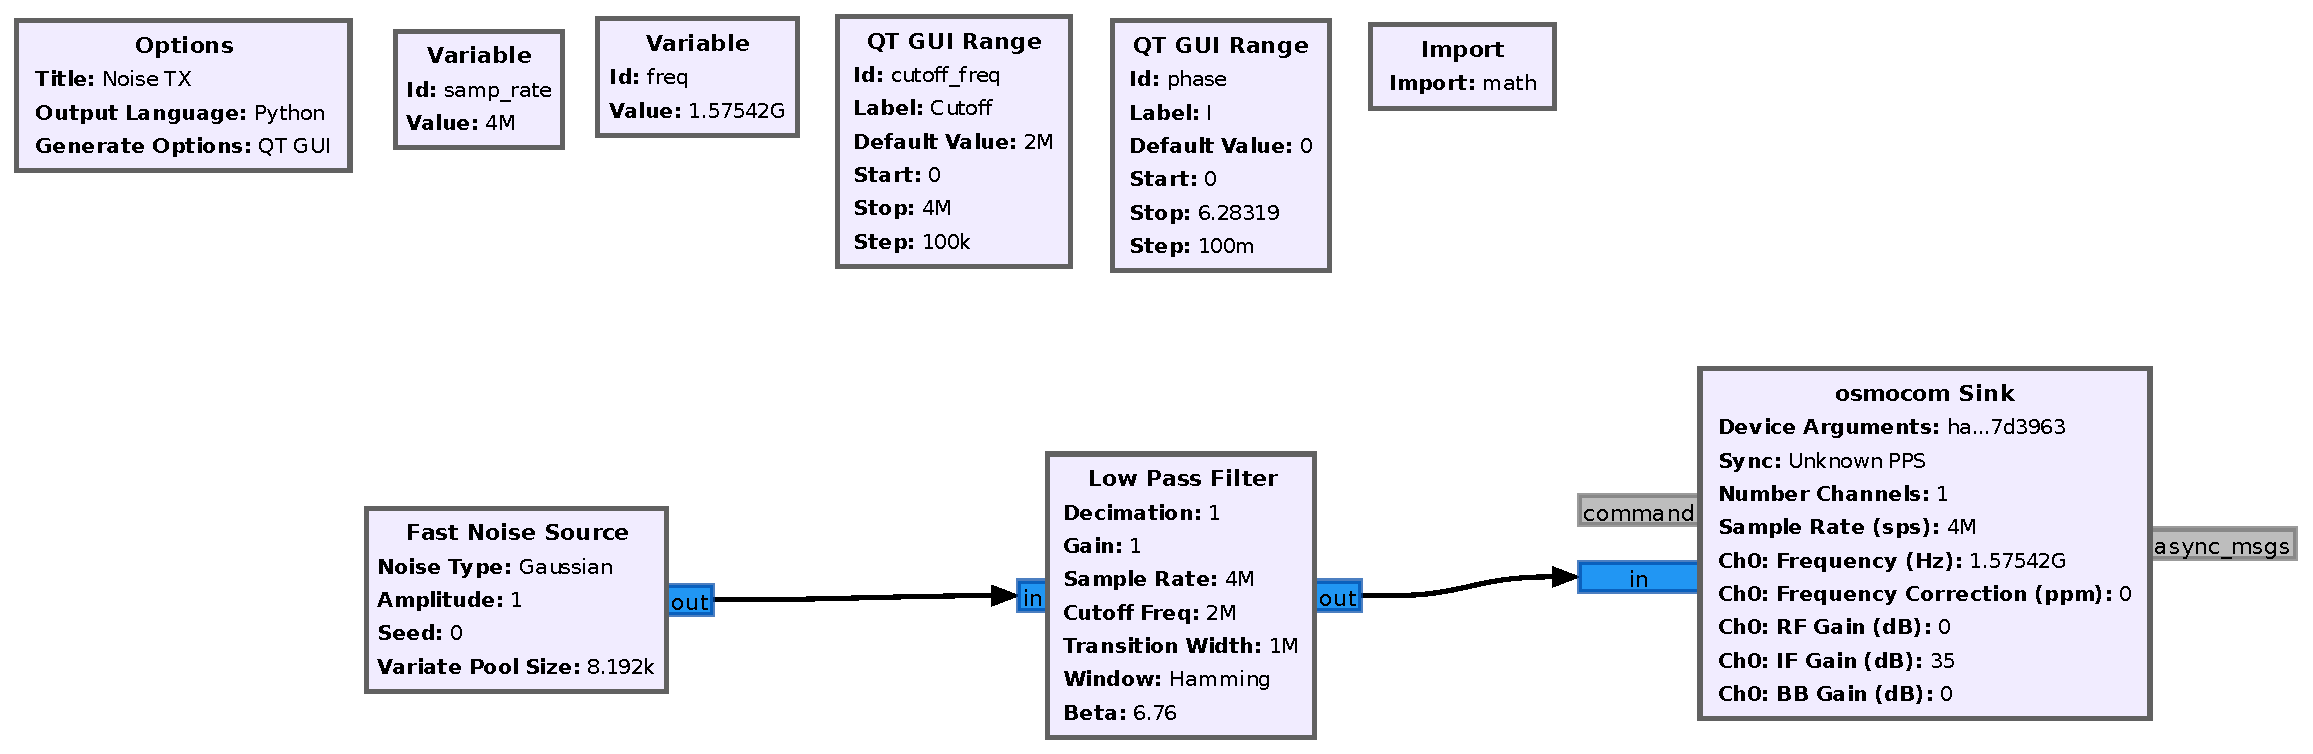
\includegraphics[angle=90, scale=0.5]{hackrf_tx_noise}
\par\end{centering}

\section{GNU Radio siųstuvo programa, pastoviam signalui generuoti}

\begin{centering}
    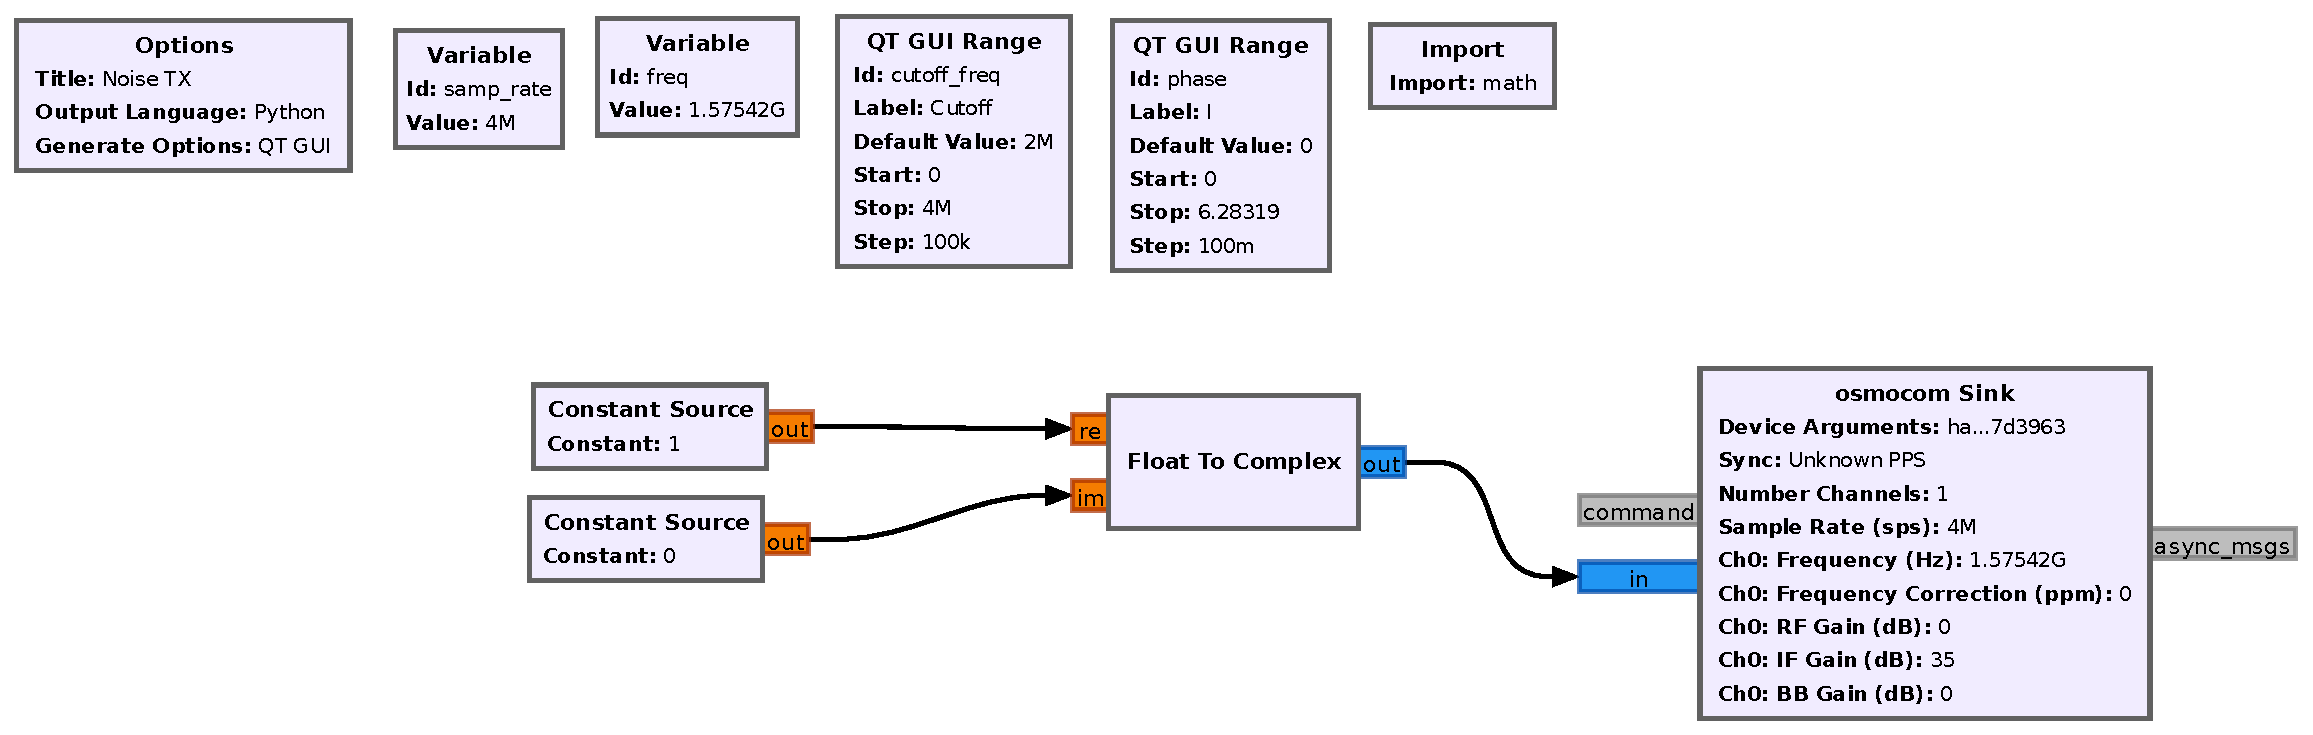
\includegraphics[angle=90, scale=0.5]{hackrf_tx}
\par\end{centering}

\section{GNU Radio programa, koreliacijos skaičiavimui}

\begin{centering}
    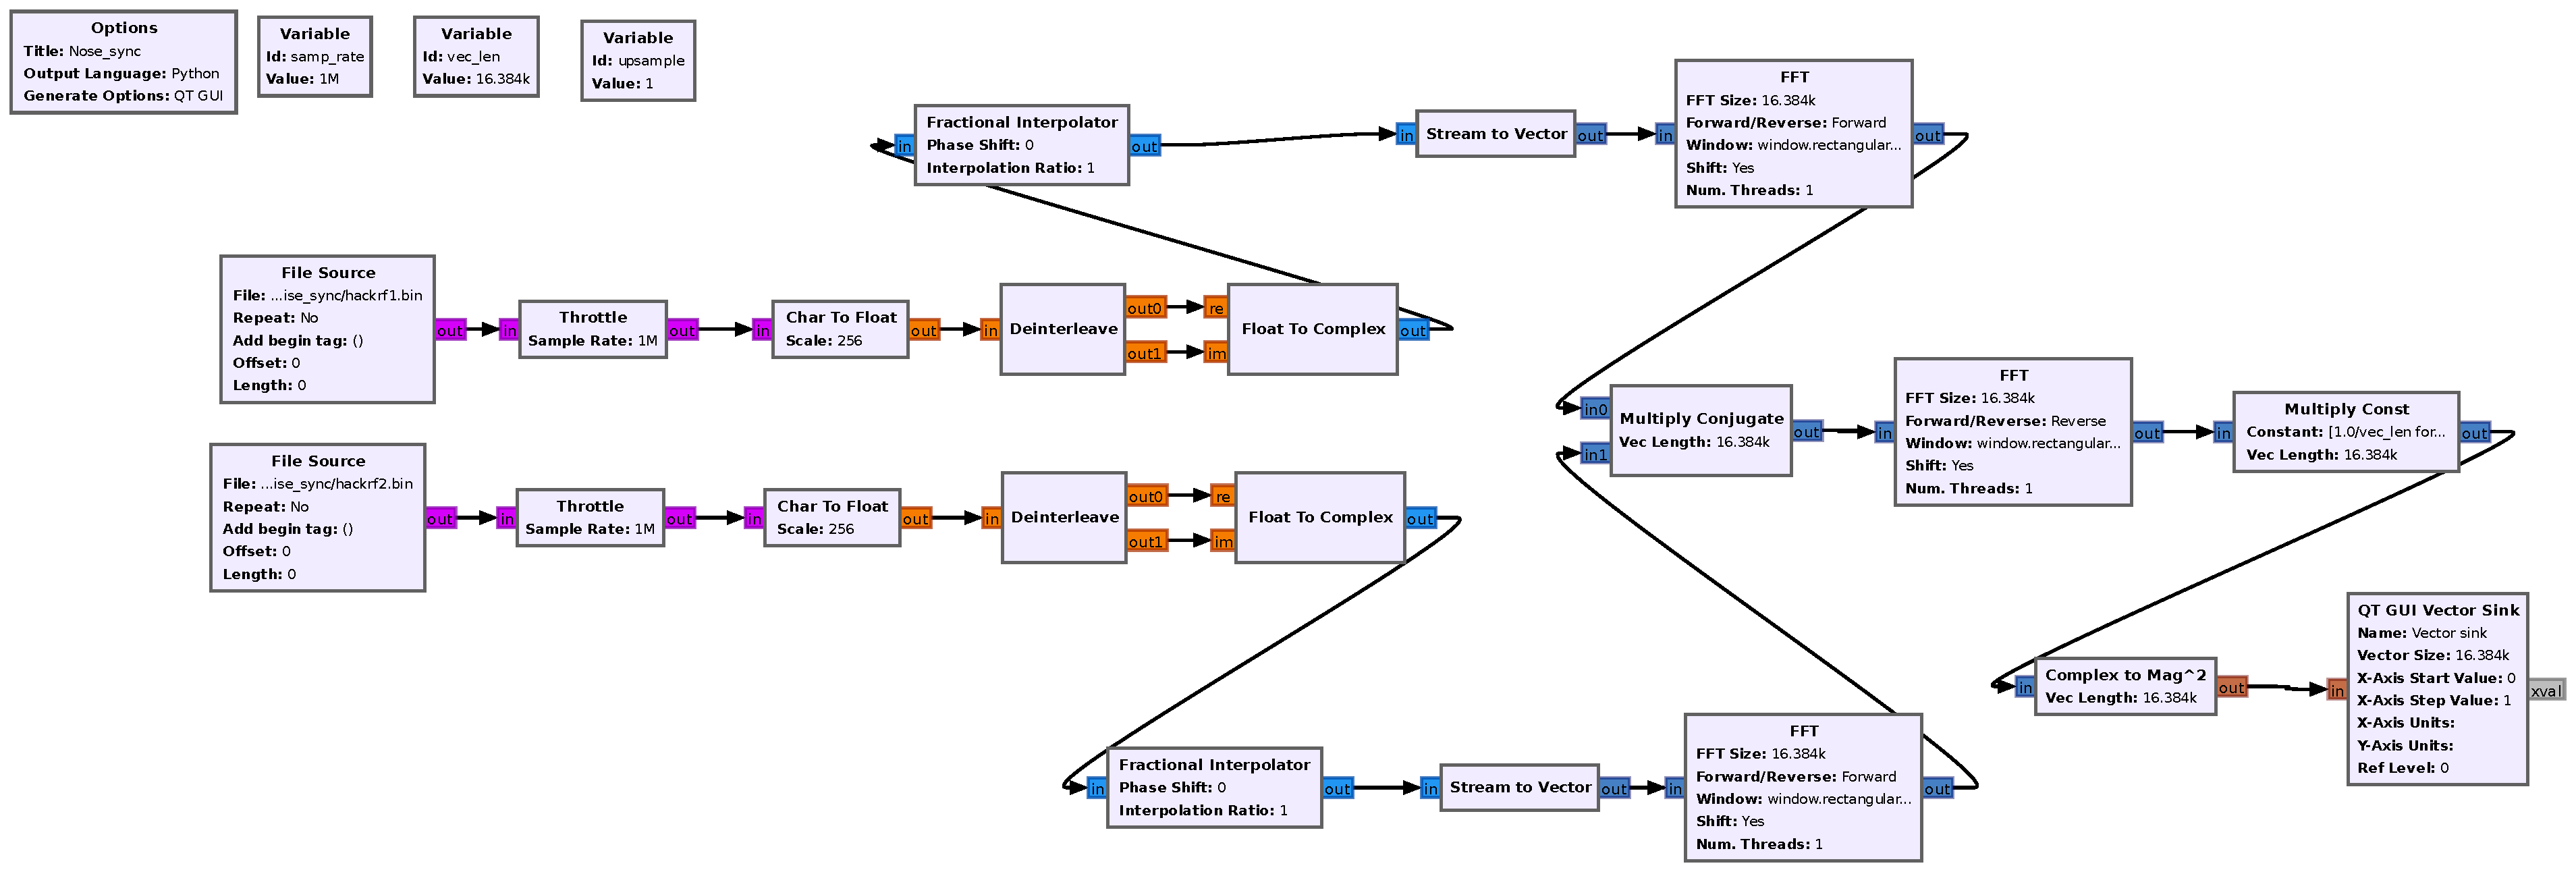
\includegraphics[angle=90, scale=0.32]{hackr_correlation}
\par\end{centering}

\section{Spindulio formavimo C++ kodas}

\definecolor{mGreen}{rgb}{0,0.6,0}
\definecolor{mGray}{rgb}{0.5,0.5,0.5}
\definecolor{mPurple}{rgb}{0.58,0,0.82}
\definecolor{backgroundColour}{rgb}{0.95,0.95,0.92}

\lstdefinestyle{CStyle}{
	basicstyle=\fontsize{5}{0}\ttfamily,
    backgroundcolor=\color{backgroundColour},   
    commentstyle=\color{mGreen},
    keywordstyle=\color{magenta},
    numberstyle=\tiny\color{mGray},
    stringstyle=\color{mPurple},
    breakatwhitespace=false,         
    breaklines=true,                 
    captionpos=b,                    
    keepspaces=true,                 
    numbers=left,                    
    numbersep=5pt,                  
    showspaces=false,                
    showstringspaces=false,
    showtabs=false,                  
    tabsize=2,
    language=C++
}

\lstinputlisting[style={CStyle}]{code.cpp}

\end{document}
